% Options for packages loaded elsewhere
% Options for packages loaded elsewhere
\PassOptionsToPackage{unicode}{hyperref}
\PassOptionsToPackage{hyphens}{url}
\PassOptionsToPackage{dvipsnames,svgnames,x11names}{xcolor}
%
\documentclass[
  letterpaper,
  DIV=11,
  numbers=noendperiod]{scrartcl}
\usepackage{xcolor}
\usepackage{amsmath,amssymb}
\setcounter{secnumdepth}{-\maxdimen} % remove section numbering
\usepackage{iftex}
\ifPDFTeX
  \usepackage[T1]{fontenc}
  \usepackage[utf8]{inputenc}
  \usepackage{textcomp} % provide euro and other symbols
\else % if luatex or xetex
  \usepackage{unicode-math} % this also loads fontspec
  \defaultfontfeatures{Scale=MatchLowercase}
  \defaultfontfeatures[\rmfamily]{Ligatures=TeX,Scale=1}
\fi
\usepackage{lmodern}
\ifPDFTeX\else
  % xetex/luatex font selection
\fi
% Use upquote if available, for straight quotes in verbatim environments
\IfFileExists{upquote.sty}{\usepackage{upquote}}{}
\IfFileExists{microtype.sty}{% use microtype if available
  \usepackage[]{microtype}
  \UseMicrotypeSet[protrusion]{basicmath} % disable protrusion for tt fonts
}{}
\makeatletter
\@ifundefined{KOMAClassName}{% if non-KOMA class
  \IfFileExists{parskip.sty}{%
    \usepackage{parskip}
  }{% else
    \setlength{\parindent}{0pt}
    \setlength{\parskip}{6pt plus 2pt minus 1pt}}
}{% if KOMA class
  \KOMAoptions{parskip=half}}
\makeatother
% Make \paragraph and \subparagraph free-standing
\makeatletter
\ifx\paragraph\undefined\else
  \let\oldparagraph\paragraph
  \renewcommand{\paragraph}{
    \@ifstar
      \xxxParagraphStar
      \xxxParagraphNoStar
  }
  \newcommand{\xxxParagraphStar}[1]{\oldparagraph*{#1}\mbox{}}
  \newcommand{\xxxParagraphNoStar}[1]{\oldparagraph{#1}\mbox{}}
\fi
\ifx\subparagraph\undefined\else
  \let\oldsubparagraph\subparagraph
  \renewcommand{\subparagraph}{
    \@ifstar
      \xxxSubParagraphStar
      \xxxSubParagraphNoStar
  }
  \newcommand{\xxxSubParagraphStar}[1]{\oldsubparagraph*{#1}\mbox{}}
  \newcommand{\xxxSubParagraphNoStar}[1]{\oldsubparagraph{#1}\mbox{}}
\fi
\makeatother


\usepackage{longtable,booktabs,array}
\newcounter{none} % for unnumbered tables
\usepackage{calc} % for calculating minipage widths
% Correct order of tables after \paragraph or \subparagraph
\usepackage{etoolbox}
\makeatletter
\patchcmd\longtable{\par}{\if@noskipsec\mbox{}\fi\par}{}{}
\makeatother
% Allow footnotes in longtable head/foot
\IfFileExists{footnotehyper.sty}{\usepackage{footnotehyper}}{\usepackage{footnote}}
\makesavenoteenv{longtable}
\usepackage{graphicx}
\makeatletter
\newsavebox\pandoc@box
\newcommand*\pandocbounded[1]{% scales image to fit in text height/width
  \sbox\pandoc@box{#1}%
  \Gscale@div\@tempa{\textheight}{\dimexpr\ht\pandoc@box+\dp\pandoc@box\relax}%
  \Gscale@div\@tempb{\linewidth}{\wd\pandoc@box}%
  \ifdim\@tempb\p@<\@tempa\p@\let\@tempa\@tempb\fi% select the smaller of both
  \ifdim\@tempa\p@<\p@\scalebox{\@tempa}{\usebox\pandoc@box}%
  \else\usebox{\pandoc@box}%
  \fi%
}
% Set default figure placement to htbp
\def\fps@figure{htbp}
\makeatother


% definitions for citeproc citations
\NewDocumentCommand\citeproctext{}{}
\NewDocumentCommand\citeproc{mm}{%
  \begingroup\def\citeproctext{#2}\cite{#1}\endgroup}
\makeatletter
 % allow citations to break across lines
 \let\@cite@ofmt\@firstofone
 % avoid brackets around text for \cite:
 \def\@biblabel#1{}
 \def\@cite#1#2{{#1\if@tempswa , #2\fi}}
\makeatother
\newlength{\cslhangindent}
\setlength{\cslhangindent}{1.5em}
\newlength{\csllabelwidth}
\setlength{\csllabelwidth}{3em}
\newenvironment{CSLReferences}[2] % #1 hanging-indent, #2 entry-spacing
 {\begin{list}{}{%
  \setlength{\itemindent}{0pt}
  \setlength{\leftmargin}{0pt}
  \setlength{\parsep}{0pt}
  % turn on hanging indent if param 1 is 1
  \ifodd #1
   \setlength{\leftmargin}{\cslhangindent}
   \setlength{\itemindent}{-1\cslhangindent}
  \fi
  % set entry spacing
  \setlength{\itemsep}{#2\baselineskip}}}
 {\end{list}}
\usepackage{calc}
\newcommand{\CSLBlock}[1]{\hfill\break\parbox[t]{\linewidth}{\strut\ignorespaces#1\strut}}
\newcommand{\CSLLeftMargin}[1]{\parbox[t]{\csllabelwidth}{\strut#1\strut}}
\newcommand{\CSLRightInline}[1]{\parbox[t]{\linewidth - \csllabelwidth}{\strut#1\strut}}
\newcommand{\CSLIndent}[1]{\hspace{\cslhangindent}#1}



\setlength{\emergencystretch}{3em} % prevent overfull lines

\providecommand{\tightlist}{%
  \setlength{\itemsep}{0pt}\setlength{\parskip}{0pt}}



 


\usepackage{needspace}
\usepackage{etoolbox}
\AtBeginEnvironment{longtable}{\Needspace{8\baselineskip}}
\KOMAoption{captions}{tableheading}
\makeatletter
\@ifpackageloaded{caption}{}{\usepackage{caption}}
\AtBeginDocument{%
\ifdefined\contentsname
  \renewcommand*\contentsname{Table of contents}
\else
  \newcommand\contentsname{Table of contents}
\fi
\ifdefined\listfigurename
  \renewcommand*\listfigurename{List of Figures}
\else
  \newcommand\listfigurename{List of Figures}
\fi
\ifdefined\listtablename
  \renewcommand*\listtablename{List of Tables}
\else
  \newcommand\listtablename{List of Tables}
\fi
\ifdefined\figurename
  \renewcommand*\figurename{Figure}
\else
  \newcommand\figurename{Figure}
\fi
\ifdefined\tablename
  \renewcommand*\tablename{Table}
\else
  \newcommand\tablename{Table}
\fi
}
\@ifpackageloaded{float}{}{\usepackage{float}}
\floatstyle{ruled}
\@ifundefined{c@chapter}{\newfloat{codelisting}{h}{lop}}{\newfloat{codelisting}{h}{lop}[chapter]}
\floatname{codelisting}{Listing}
\newcommand*\listoflistings{\listof{codelisting}{List of Listings}}
\makeatother
\makeatletter
\makeatother
\makeatletter
\@ifpackageloaded{caption}{}{\usepackage{caption}}
\@ifpackageloaded{subcaption}{}{\usepackage{subcaption}}
\makeatother
\definecolor{quarto-callout-cnj-color}{HTML}{558B2F}
\definecolor{quarto-callout-cnj-color-frame}{HTML}{558B2F}
\definecolor{quarto-callout-cor-color}{HTML}{00838F}
\definecolor{quarto-callout-cor-color-frame}{HTML}{00838F}
\definecolor{quarto-callout-exr-color}{HTML}{FFA500}
\definecolor{quarto-callout-exr-color-frame}{HTML}{FFA500}
\definecolor{quarto-callout-remark-color}{HTML}{AD1457}
\definecolor{quarto-callout-remark-color-frame}{HTML}{AD1457}
\definecolor{quarto-callout-prp-color}{HTML}{827717}
\definecolor{quarto-callout-prp-color-frame}{HTML}{827717}
\definecolor{quarto-callout-proof-color}{HTML}{37474F}
\definecolor{quarto-callout-proof-color-frame}{HTML}{37474F}
\definecolor{quarto-callout-exm-color}{HTML}{6A1B9A}
\definecolor{quarto-callout-exm-color-frame}{HTML}{6A1B9A}
\definecolor{quarto-callout-solution-color}{HTML}{4E342E}
\definecolor{quarto-callout-solution-color-frame}{HTML}{4E342E}
\definecolor{quarto-callout-def-color}{HTML}{1B5E20}
\definecolor{quarto-callout-def-color-frame}{HTML}{1B5E20}
\definecolor{quarto-callout-lem-color}{HTML}{1565C0}
\definecolor{quarto-callout-lem-color-frame}{HTML}{1565C0}
\usepackage{bookmark}
\IfFileExists{xurl.sty}{\usepackage{xurl}}{} % add URL line breaks if available
\urlstyle{same}
% fallback for those not using the hyperref driver hyperxmp:
\makeatletter
\@ifundefined{xmpquote}{\newcommand{\xmpquote}[1]{#1}}{}
\makeatother
\hypersetup{
  pdftitle={Quarto Manuscript Template},
  pdfauthor={Your Name},
  pdfkeywords={\xmpquote{template}, \xmpquote{quarto}, \xmpquote{manuscript}},
  colorlinks=true,
  linkcolor={blue},
  filecolor={Maroon},
  citecolor={Blue},
  urlcolor={Blue},
  pdfcreator={LaTeX via pandoc}}


\title{Quarto Manuscript Template}
\author{Your Name}
\date{Last modified: 2026-10-08 21:57:43 (UTC)}
\begin{document}
\maketitle
\begin{abstract}
This is a template for creating manuscripts with Quarto. Replace this
abstract with your own summary of the work: the research question,
methods, key findings, and conclusions. Aim for 150--250 words for most
journals.
\end{abstract}


\section{Introduction}\label{sec-intro}

This is a Quarto manuscript template. The manuscript is available in
multiple formats:

\begin{itemize}
\tightlist
\item
  \textbf{HTML}: An interactive web version with table of contents and
  linked cross-references
\item
  \textbf{PDF}: A print-ready document suitable for journal submission
\item
  \textbf{DOCX}: A Microsoft Word document for collaborators who prefer
  tracked changes
\item
  \textbf{JATS XML}: A structured format required by some journals and
  preprint servers
\end{itemize}

Cite references with \texttt{@citationkey} (Author 2024) or in
parentheses (Author and Coauthor 2024).

\subsection{Background}\label{background}

Add background and motivation here. Cross-reference sections with
\texttt{@sec-methods} (renders as Section~\ref{sec-methods}).

\section{Methods}\label{sec-methods}

Describe your study design, data sources, and analysis approach here.

\subsection{Data}\label{data}

You can include inline R code: the square root of 2 is 1.4142.

\subsection{Analysis}\label{analysis}

Code chunks execute and embed results:

Supplementary analyses live in a separate notebook
(\texttt{notebooks/supplementary-analysis.qmd}) and are embedded in the
HTML output automatically.

\section{Results}\label{sec-results}

Present your findings here. Reference figures with \texttt{@fig-example}
(Figure~\ref{fig-example}) and tables with \texttt{@tbl-summary}
(Table~\ref{tbl-summary}).

\protect\phantomsection\label{cell-fig-example}
\begin{figure}[H]

\centering{

\pandocbounded{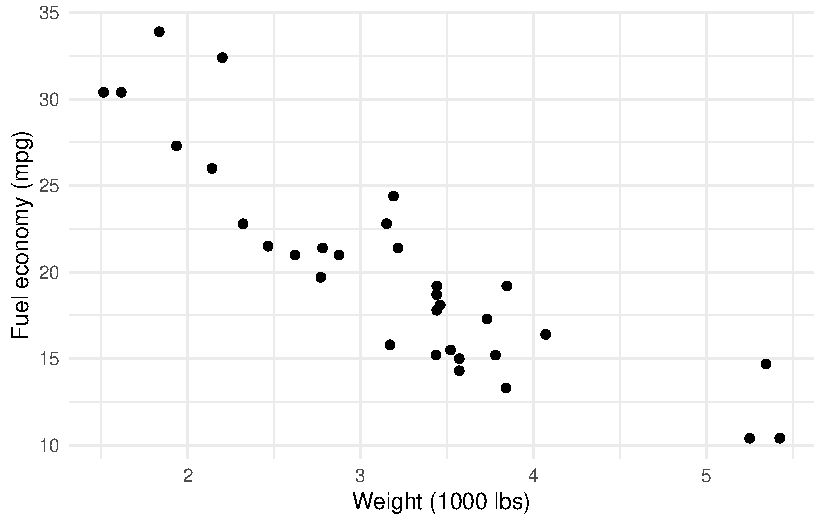
\includegraphics[keepaspectratio,alt={Scatter plot showing a negative relationship between car weight (x-axis) and fuel economy in miles per gallon (y-axis).}]{index_files/figure-pdf/fig-example-1.pdf}}

}

\caption{\label{fig-example}Fuel economy vs.~weight for 32 cars.}

\end{figure}%

\textsubscript{Source:
\href{https://Morrison-Lab.github.io/qmt/index.qmd.html}{Article
Notebook}}

\section{Discussion}\label{sec-discussion}

Interpret your results, address limitations, and describe implications.

\section{Conclusion}\label{sec-conclusion}

Summarize the key findings and their significance.

\section*{References}\label{references}
\addcontentsline{toc}{section}{References}

\protect\phantomsection\label{refs}
\begin{CSLReferences}{1}{1}
\bibitem[\citeproctext]{ref-example2024}
Author, Example. 2024. \emph{Example Book Title}. Example Publisher.
\url{https://doi.org/10.1007/978-3-319-24277-4}.

\bibitem[\citeproctext]{ref-example-article2024}
Author, Example, and Another Coauthor. 2024. {``Example Article
Title.''} \emph{Example Journal} 10 (1): 1--10.
\url{https://doi.org/10.1038/nature12373}.

\end{CSLReferences}

This sentence tests the PR preview and will not be merged.




\end{document}
